\documentclass[sigconf]{acmart}

\AtBeginDocument{%
  \providecommand\BibTeX{{%
    Bib\TeX}}}

\acmConference[ITSEC]{IT-Security Seminar}{WiSe 2023/24}{Heidelberg}
\begin{document}
\title{PQC WireGuard as a new VPN}
\subtitle{WireGuard + Rosenpass}

\author{Philip Kastura-Sahl}
\email{philip.kastura-sahl@stud.uni-heidelberg.de}
\affiliation{%
  \institution{Ruprecht-Karls-Universität Heidelberg}
  \city{Heidelberg}
  \country{Germany}
}

\renewcommand{\shortauthors}{Philip Kastura-Sahl}

\begin{abstract}
  With the advance of quantum computers, security researchers face the challenge of securing their data against \textit{"Harvest now, decrypt later"-attacks} that could become available in the future. Shor's algorithm\cite{Shor_1997}, when implemented on a sufficiently powerful quantum computer, could be used to break many public-key cryptography schemes. Rosenpass aims to provide a \textit{post-quantum-secure authenticated key exchange} that works in a \textit{hybrid post-quantum security scheme} together with WireGuard. Due to the ongoing development of Post-quantum-Ciphers, Rosenpass is implemented to provide hybrid post-quantum security in tandem with WireGuard\cite{Rosenpass-about}.
\end{abstract}

\begin{CCSXML}
  <ccs2012>
  <concept>
  <concept_id>10002978.10003014.10003015</concept_id>
  <concept_desc>Security and privacy~Security protocols</concept_desc>
  <concept_significance>300</concept_significance>
  </concept>
  <concept>
  <concept_id>10002978.10003014.10003016</concept_id>
  <concept_desc>Security and privacy~Web protocol security</concept_desc>
  <concept_significance>500</concept_significance>
  </concept>
  <concept>
  <concept_id>10002978.10002979.10002981.10011745</concept_id>
  <concept_desc>Security and privacy~Public key encryption</concept_desc>
  <concept_significance>500</concept_significance>
  </concept>
  <concept>
  <concept_id>10002978.10002979.10002980</concept_id>
  <concept_desc>Security and privacy~Key management</concept_desc>
  <concept_significance>500</concept_significance>
  </concept>
  <concept>
  <concept_id>10002978.10002986.10002988</concept_id>
  <concept_desc>Security and privacy~Security requirements</concept_desc>
  <concept_significance>100</concept_significance>
  </concept>
  </ccs2012>
\end{CCSXML}

\ccsdesc[300]{Security and privacy~Security protocols}
\ccsdesc[500]{Security and privacy~Web protocol security}
\ccsdesc[500]{Security and privacy~Public key encryption}
\ccsdesc[500]{Security and privacy~Key management}
\ccsdesc[100]{Security and privacy~Security requirements}

\keywords{Post-quantum cryptography, Key-Encapsulation Method, Rosenpass, WireGuard, Crystals-Kyber, NIST}

\begin{teaserfigure}
  \centering
  
\includegraphics[width=\textwidth]{graphics/rosenpass+wireguard.pdf}
\end{teaserfigure}

\received[Talk]{18 January 2024}
\received[Paper]{31 March 2024}

\maketitle

%%%%%%%%%%%%%%%%%%%%%%%%%%%%%%%%%%%%%%%%%%%%%%%%%%%%%%%%%%%%%%%%%%%%%%%%%%%%%%%%%%%%%%%%%%%%%%%%%%%%%%%%%%%%%%%%%%%%%%%%%%%%%%%%%%%%%%%%%%%%%%%%%%%%%%%%%%%%%%%%%%%%
% Begin Document
%%%%%%%%%%%%%%%%%%%%%%%%%%%%%%%%%%%%%%%%%%%%%%%%%%%%%%%%%%%%%%%%%%%%%%%%%%%%%%%%%%%%%%%%%%%%%%%%%%%%%%%%%%%%%%%%%%%%%%%%%%%%%%%%%%%%%%%%%%%%%%%%%%%%%%%%%%%%%%%%%%%%

\section{Introduction}
Shor's Algorithm, developed in 1994 by Peter Shor, is one of the few known algorithms that could be used to break existing public key cryptography such as RSA and some Diffie-Hellman variants. With the rise of ever more powerful quantum computers, security researchers are facing the possibility of traditional \textit{pre-quantum cryptography} becoming insecure. The Open Quantum Safe Project\cite{open-quantum-safe} \& NIST\footnote{NIST -- National Institute of Standards and Technology} aim to improve and standardize \textit{post-quantum cryptography} to the point of it being able to supersede existing schemes that would be deemed insecure using sufficiently powerful quantum computers. \\
PQ-WireGuard\cite{cryptoeprint:2020/379} first modified WireGuard and implemented new PQ\footnote{pq -- post-quantum} forward secrecy \& pq Authentication by replacing the Diffie-Hellman handshake with a key-encapsulation mechanism\footnote{KEM -- key-encapsulation mechanism}.

\subsection{WireGuard \& Rosenpass}
WireGuard is a modern VPN that intends to be more performant than OpenVPN, whilst being able to run on a variety of computers and platforms\cite{WireGuard}. Rosenpass functions as an Add-on to WireGuard, adding PQC\footnote{PQC -- post-quantum cryptography} whilst keeping the established security intact. Whilst some WireGuard implementations are considered complete\cite{wg-repos}, Rosenpass is still under development\cite{rosenpass}. Apart from implementing PQC, Rosenpass also implements a statless responder to protect against replay attacks of the first protocol message.

\subsection{Problem Definition}
Even though Quantum Computers don't yet have a sufficient number of qubits, data could be harvested already, making it vulnerable to decryption attacks in the future, a surveillance strategy known as \textit{Harvest now, decrypt later}. Yet PQC has not yet reached the point of adoption to be replacing pre-quantum cryptography, as seen in the Post-Quantum Cryptography Standardization effort where algorithms such as SIDH have been eliminated due to major security flaws in their design\cite{cryptoeprint:2022/975}. Therefore, Rosenpass has been designed to implement Hybrid PQC\cite{cryptoeprint:2022/1225}, Rosenpass providing encryption deemed the most post-quantum resistant and working together with the known to be pre-quantum secure WireGuard. The handshake between WireGuard and Rosenpass as well as the individual connections between Rosenpass and WireGuard Clients and Server needed to be designed in such a way that neither one of the ciphers could be broken alone so that a potential attacker would need to always attack both ciphers.


\section{Ciphers}
The Rosenpass developers have chosen a combination of Classic McEliece and CRYSTALS-Kyber, notably finalists of the NIST Post-Quantum Cryptography Standardization effort\cite{pqc-standardization}. While symmetric ciphers are generally considered to be secure, not all asymmetric ciphers are equally vulnerable to Shor's algorithm.

\subsection{KEM vs. NIKE}
Established asymmetric ciphers \textit{Non-Interactive Key Exchange}, as the name implies, this enables two parties to know each other's public keys and agree on a symmetric shared key without requiring any interaction\cite{cryptoeprint:2012/732}. While a NIKE\footnote{NIKE -- Non-Interactive Key Exchange} is not inherently insecure against attacks by quantum computers, PQC usually relies on a \textit{Key encapsulation mechanism}. KEMs\footnote{KEM -- Key encapsulation mechanism} are considered a more viable solution, because they are able to provide both pq-resistance as well as today's security guarantees. Hybrid PQC can be implemented using KEMs by using a combiner, which enables the use of multiple algorithms while keeping the scheme secure as long as one of the algorithms remains secure\cite{cryptoeprint:2018/903}.

\subsection{Classic McElice}
Classic McEliece decodes linear codes using an algorithm that introduces errors and derives a public key using \textit{binary goppa codes}. Binary goppa codes are error correcting code from the class of general Goppa codes, they can be used to encode messages whilst introducing errors\cite{1055873}. The Classic McEliece public keys tend to be larger than other ciphers, at least 261120 Bytes\textsuperscript{(for mceliece348864)}, whereas their ciphertext is 96 Bytes\textsuperscript{(for mceliece348864)}.

\subsection{Kyper}
\textit{Lattice-based ciphers} such as CRYSTALS-Kyber are based on \textit{lattice problems} such as the \textit{Shortest Vector Problem} and \textit{Learning with Errors}\cite{10.1145/1568318.1568324}. \\
The SVP\footnote{SVP -- Shortest Vector Problem} is considered solved if the shortest possible vector measured by a given norm is found for a given lattice. Algorithms to solve SVP such as LLL\footnote{LLL -- Lenstra–Lenstra–Lovász} lattice basis reduction algorithm often require polynomial time \[\mathcal{O}(d^5 n \log^3 B)\], where \[B = \max(\left\| b_1 \right\|_2, \left\| b_2 \right\|_2, \dots , \left\| b_d \right\|_2)\]\cite{doi:10.1137/070705702}, due to their complexity SVP is considered to be secure against traditional and quantum computers\cite{915326}. \\
LWE\footnote{LWE -- Learning with Errors} is a problem of differentiating random from uniform linear equations\cite{10.1145/2535925}, it can be used to obfuscate the secret by introducing noise into the linear equations used inside the cipher.


\section{Implementation}
The Rosenpass Team has chosen to develop Rosenpass alongside WireGuard as an Add-on. Contrary to its predecessor WireGuard-PQ, Rosenpass only implements the post-quantum side and relies on WireGuard to provide sufficient pre-quantum security such that the entire system works as a hybrid post-quantum security scheme. This approach requires the development teams of both Rosenpass and WireGuard to work together to ensure compatibility, as well as administrators and users willingness to keep their installed Rosenpass and WireGuard versions compatible. Yet, choosing this approach enables the Rosenpass Team to focus solely on the development and proofing of Rosenpass without the technological depth of maintaining the pre-quantum security.

\subsection{Proof}
The Rosenpass Team provides a symbolic analysis using the \textit{proverif} tool. Using proverif an automated security analysis can be executed on the provided Rosenpass implementations. A cryptographic proof of security is currently worked on, but has not yet been published\cite{rosenpass}\textsuperscript{[As of 10.03.2024]}.

%\subsection{Audit}

\subsection{Key Exchange}
The Rosenpass Handshake works much like the traditional WireGuard handshake, needing to be refreshed every 2 minutes. Apart from using PQC, it differentiates itself by ensuring Non-Interruptibility through the use of a \textit{Biscuit}. WireGuard provides Non-Interruptibility by including a Timestamp, the Rosenpass Team has wrapped the \textit{Responder State} inside a Cookie, dubbed \textit{Biscuit}\cite{rosenpass}. \\
For a visualization, see \ref{appendix:exchange}.

\subsection{WireGuard-Rosenpass Handshake}
The Handshake between WireGuard and Rosenpass ensures that the Connection remains secure at all times. When the connection between WireGuard and its Client gets disconnected the entire communication naturally breaks down, Rosenpass is implemented to provide a \textit{PSK} to WireGuard. When the Rosenpass Handshake fails, the PSK upon which WireGuard depends when working together with Rosenpass gets corrupted, prompting WireGuard to pause any communication, until both Handshakes work again\cite{rosenpass}.\\
For a visualization, see \ref{appendix:handshake}.


\section{Conclusion}
Rosenpass poses a viable solution to secure networks against \textit{"Harvest now, decrypt later"-attacks}, yet there is still a need for further development. A Proof of cryptographic security is still under development and the security of existing PQC remain unclear.

%%%%%%%%%%%%%%%%%%%%%%%%%%%%%%%%%%%%%%%%%%%%%%%%%%%%%%%%%%%%%%%%%%%%%%%%%%%%%%%%%%%%%%%%%%%%%%%%%%%%%%%%%%%%%%%%%%%%%%%%%%%%%%%%%%%%%%%%%%%%%%%%%%%%%%%%%%%%%%%%%%%%

\begin{acks}
I would like to express my sincere gratitude to the following individuals and teams who have contributed to the completion of this document:

\begin{itemize}
  \item Prof. Dr. Heuveline \& Mr. Machmeier for their guidance and support throughout the research and writing process.
  \item The WireGuard \& Rosenpass teams for their respective Projects, their novice-friendly documentation, and beginner-friendly explainers.
\end{itemize}

I am truly thankful for their dedication and collaboration, which has significantly enriched the quality of this work.
\end{acks}

\bibliographystyle{ACM-Reference-Format}
\bibliography{sources}

%%%%%%%%%%%%%%%%%%%%%%%%%%%%%%%%%%%%%%%%%%%%%%%%%%%%%%%%%%%%%%%%%%%%%%%%%%%%%%%%%%%%%%%%%%%%%%%%%%%%%%%%%%%%%%%%%%%%%%%%%%%%%%%%%%%%%%%%%%%%%%%%%%%%%%%%%%%%%%%%%%%%

\appendix

\section{Implementation}

\subsection{Key Exchange}\label{appendix:exchange}
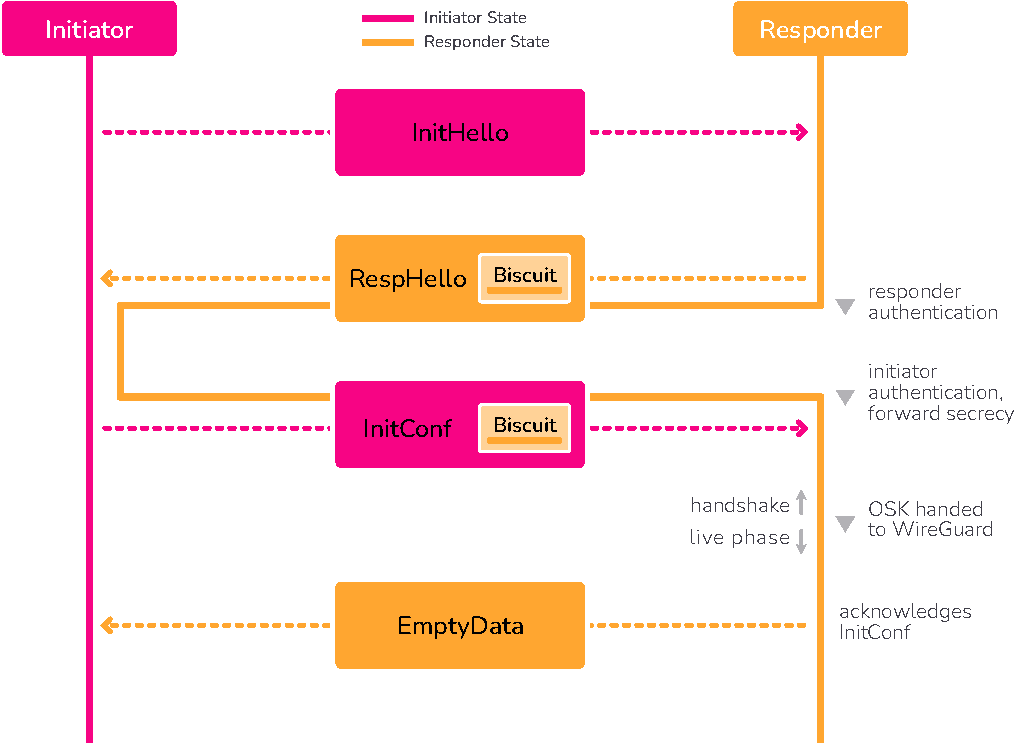
\includegraphics[height=.35\textwidth]{graphics/rosenpass-wp-key-exchange-protocol-rgb.pdf}

\subsection{WireGuard-Rosenpass Handshake}\label{appendix:handshake}
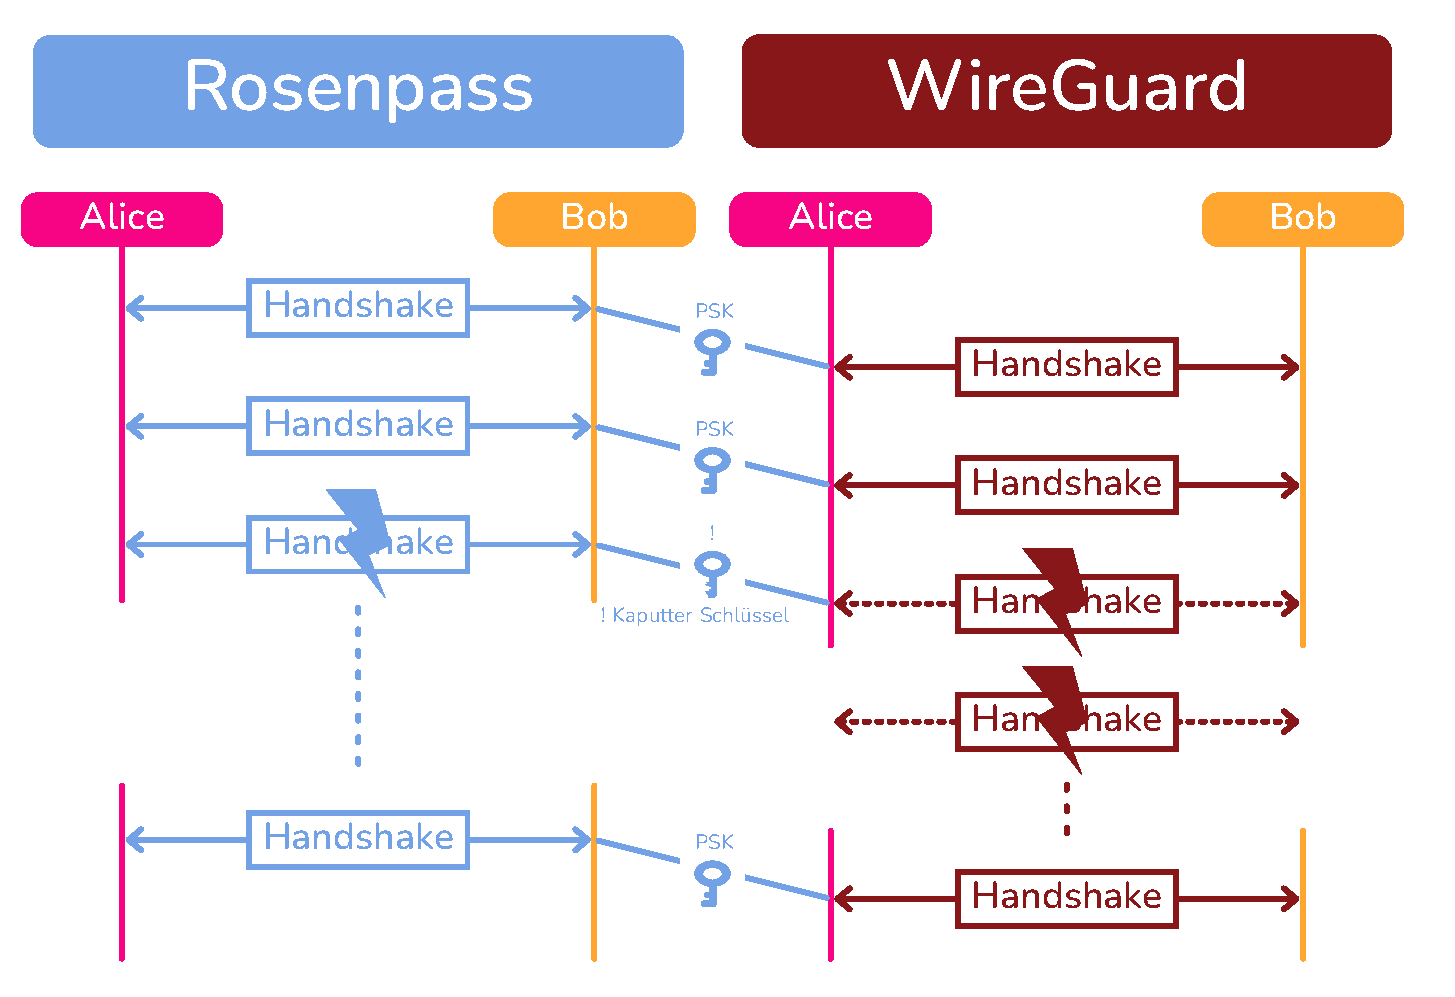
\includegraphics[height=.35\textwidth]{assets/rosenpass-wireguard.png}

%%%%%%%%%%%%%%%%%%%%%%%%%%%%%%%%%%%%%%%%%%%%%%%%%%%%%%%%%%%%%%%%%%%%%%%%%%%%%%%%%%%%%%%%%%%%%%%%%%%%%%%%%%%%%%%%%%%%%%%%%%%%%%%%%%%%%%%%%%%%%%%%%%%%%%%%%%%%%%%%%%%%
% End Document
%%%%%%%%%%%%%%%%%%%%%%%%%%%%%%%%%%%%%%%%%%%%%%%%%%%%%%%%%%%%%%%%%%%%%%%%%%%%%%%%%%%%%%%%%%%%%%%%%%%%%%%%%%%%%%%%%%%%%%%%%%%%%%%%%%%%%%%%%%%%%%%%%%%%%%%%%%%%%%%%%%%%

\end{document}
\endinput
